\documentclass{book}

% page geometry
\usepackage[
    a4paper,
    % left and right margin
    inner=1.2in,
    outer=1.2in,
    % top and bottom margin
    vmargin=1in, 
]{geometry}
%% page geometry END

%% font settings
\usepackage{fontspec, newunicodechar, polyglossia}

\setsansfont{DejaVu Sans}[Scale=MatchLowercase, Ligatures=TeX]
\setmonofont{DejaVu Sans Mono}[Scale=MatchLowercase]
\renewcommand{\familydefault}{\sfdefault}
%%
\usepackage{lipsum} % random text



%% pkg for make title page
\usepackage{geometry}
\usepackage{graphicx} % insert img
\usepackage[some]{background}

\DeclareFixedFont{\MainHeading}{T1}{phv}{b}{n}{1.5cm}
\DeclareFixedFont{\SecondaryHeading}{T1}{phv}{b}{n}{0.8cm}
\backgroundsetup{
scale=1,
angle=0,
opacity=1,
contents={
\begin{tikzpicture}[remember picture,overlay]
  \draw [path picture={
    \node at (path picture bounding box.center){
      % remember to adjust bg img height
      %   when you changed the box size
      % now: 11cm - 4cm = 7cm
      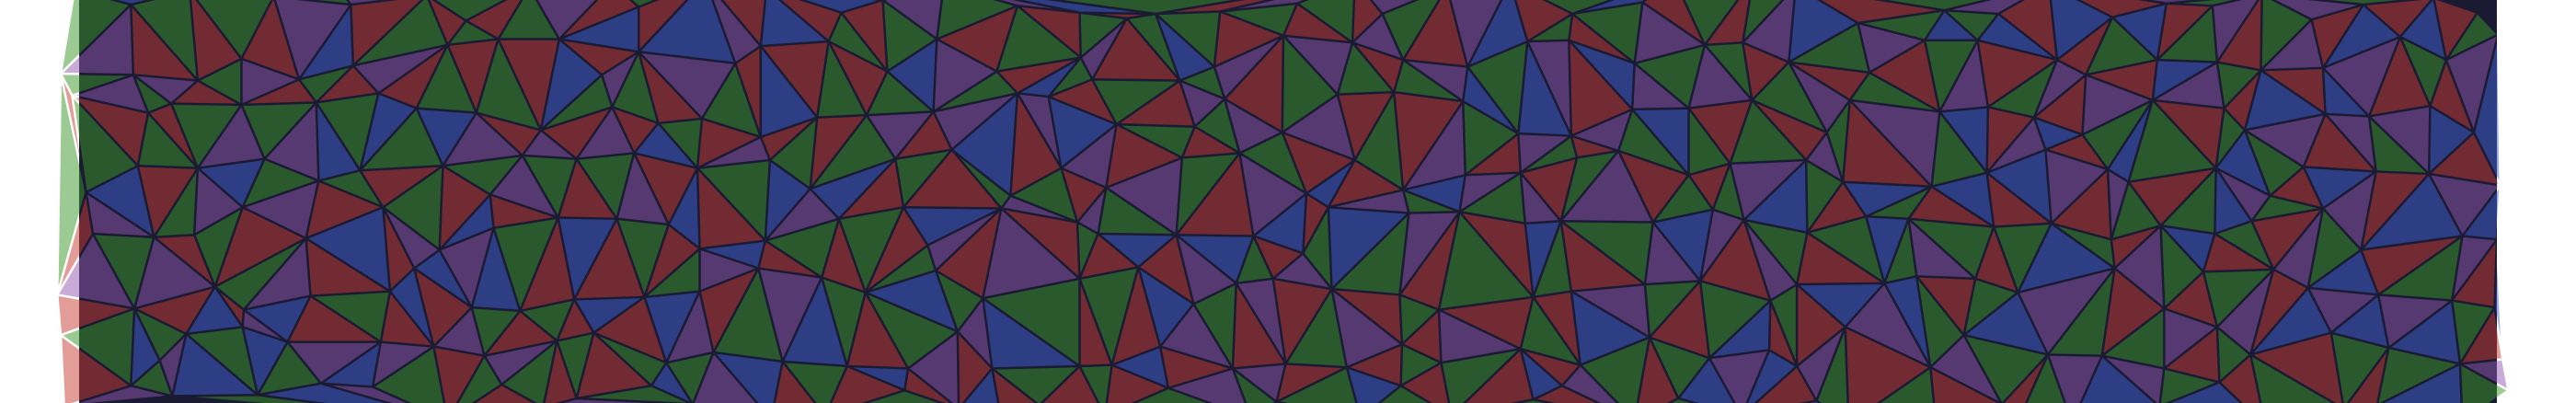
\includegraphics[height=7cm]{backsplash}
  };}] (-0.5\paperwidth,4cm) rectangle (0.5\paperwidth,11cm);
\end{tikzpicture}
}}
%% title page END

\begin{document}


\newgeometry{left=1cm,right=1cm}
\begin{titlingpage}
\BgThispage

%% Main Heading & Secondary Heading
\vspace*{2cm}\noindent
\textcolor{white}{ \MainHeading The Julia Language } 
\\[0.6cm]
\textcolor{white}{
    \SecondaryHeading A fresh approach to technical computing.
}
\vspace*{3cm}\par\noindent


%% other content: logo, doc name, time
\begin{center}

% logo

\includegraphics[width=0.3\textwidth]{./titlepage/logo} 
\\[1.5cm]

% Title
{ \SecondaryHeading Julia DEV Documentation} 
\\[1.5cm]
{ \huge The Julia Project}
\\[0.5cm]
{ \huge \today }

\end{center} 

\end{titlingpage}
\restoregeometry

\tableofcontents
\clearpage

\chapter{chap 01}
\section{A section}
\lipsum

\end{document}